%%%%%%%%%%%%%%%%%%%%%%%%%%%%%%%%
% Mein Standart Latex Document %
%%%%%%%%%%%%%%%%%%%%%%%%%%%%%%%%
\documentclass[12pt,a4paper,one side]{article}%Schriftgröße, Layout, Papierformat, Art des Dokumentes

\parindent=0pt
\parskip=1ex
\usepackage[inner=3cm,outer=2cm,top=2cm,bottom=2cm,includeheadfoot]{geometry}%Einstellungen der Seitenränder

\usepackage[utf8]{inputenc}%Umlaute ermöglichen
\usepackage{ngerman}%neue Rechtschreibung
\usepackage{color} %Farben ermoeglichen
\usepackage{fancyhdr}
\usepackage{hyperref}%Links Einfuegen
\usepackage{graphicx}
\usepackage{lipsum}
\usepackage{DavidMacros}
\usepackage{mhchem}
\usepackage{tikz}
\usepackage{tabularx}
\usepackage{cclicenses}

%%%Chemie Packages
%\usepackage{mhchem}
%\usepackage{chemfig}

%%%Channge To TT Style
%\everymath={\tt }
%\renewcommand{\familydefault}{\ttdefault}

\hypersetup{
    pdftitle = {Strahlenschutz - Formelsammlung},
    pdfauthor = {Pni0}
}


%%%Farbdefinitionen
\definecolor{grau}{gray}{.5}% Grau
\definecolor{hellgrau}{gray}{.8}% Hellgrau
\definecolor{hellhellgrau}{gray}{.965}% HellHellgrau

%%%Fancy Kopf und Fuß zeilen
\pagestyle{fancy}%Kopf- und Fußzeile
\fancyhf{}
\fancyhead[RO,LE]{\nouppercase{\leftmark}}%Kopfzeile rechts bzw. außen
\renewcommand{\headrulewidth}{0.5pt}%Linie oben
\fancyhead[LO,RE]{\nouppercase{\Title}}
\fancyfoot[RO,LE]{-~\thepage~-~}%Fußzeile rechts bzw. außen
\renewcommand{\footrulewidth}{0.5pt}%Linie unten

\fancypagestyle{plain}{%Plain Seiten Style erneuern
\fancyhead[RO,LE]{\nouppercase{\leftmark}}%Kopfzeile rechts bzw. außen
\fancyhead[LO,RE]{\nouppercase{\Title}}
\renewcommand{\headrulewidth}{0.5pt}%Linie oben
\fancyfoot[RO,LE]{-~\thepage~-~}%Fußzeile rechts bzw. außen
\renewcommand{\footrulewidth}{0.5pt}%Linie unten
}

%%%Hyperref Setup
\hypersetup{pdftex=true, colorlinks=true, breaklinks=true, linkcolor=black, menucolor=black, pagecolor=black, urlcolor=black}
%\hypersetup{pdftex=true, colorlinks=true, breaklinks=true, linkcolor=blue, menucolor=blue, pagecolor=blue, urlcolor=blue}

%%%
%\newcommand{\wichtig}[1]{{\bf #1}}%Neuse commando Wichtig zur textvormatierung
\newcommand{\fwichtig}[1]{%Umrahmen von Formeln
\begin{center}\fcolorbox{grau}{hellhellgrau}{
\begin{tabular}{l}
#1
\end{tabular}}\end{center}
}

\newcommand{\bruch}[2]{\frac{\displaystyle{#1}}{\displaystyle{#2}}}



%%%%%%%%%%%%%%FrontePage info%%%%%%%%%%%%%%%%%%%%%%%%%%%%%%%%%%%%%%%
\newcommand{\Title}{Strahlenschutz}
\newcommand{\SubTitle}{Formelsammlung}
\newcommand{\TheAuthor}{}
\newcommand{\Datum}{\today}
\newcommand{\Licence}{\cc 0}

\newcommand{\Version}{}
\newcommand{\Status}{}
%%%%%%%%%%%%%%%%%%%%%%%%%%%%%%%%%%%%%%%%%%%%%%%%%%%%%%%%%%%%%%%%%%%%
\setcounter{tocdepth}{2}

\begin{document}
\thispagestyle{empty}
\begin{center}

{\textcolor{grau} \TheAuthor} \hfill {\textcolor{grau} \Datum}
~\vfill
{\Huge\sc \Title}\\
\textcolor{hellgrau}{\rule{\textwidth}{1ex}}
{\Large {\SubTitle}}\\
\vfill
{\textcolor{grau} \Licence} \hfill  {\textcolor{grau} \Version}{\textcolor{grau} \Status}
\end{center}
\clearpage
\tableofcontents
\renewcommand{\thepage}{\Roman{page}}
\setcounter{page}{1}
\clearpage
\renewcommand{\thepage}{\arabic{page}}
\setcounter{page}{1}

%%%%%%%%%%%%%%%%%%%%%%%%%%%%
% Physikalische Grundlagen %
%%%%%%%%%%%%%%%%%%%%%%%%%%%%

\section{Physikalische Grundlagen}
\subsection{Röntgenstrahlung}
In einer Röhre wird die Anode (Röntgen-Target)  mit schnellen Elektronen Beschossen.
Beim Aufprall eines Elektrons wird dieses abgebremst und es entsteht ein Photon mit der Frequenz $f_{\rm(U_B)}$.
Diese elektromagnetische Strahlung heisst \wichtig{Bremsstrahlung}.
Durch die unterschiedliche Abbremsung entsteht der sogenannte Bremsbuckel im Wellenlängen Spektrum.\\
$hf_{\rm g} = E = eU_{\rm B}$\\
\fwichtig{\wichtig{Grenzwellenlänge: }$\lambda_{\rm g} = \frac{c}{f_{\rm g}} = \frac{hc}{eU_{\rm B}} = \frac{1234nm}{U_{\rm B}}$}
\subsubsection*{Absorptionsgesetz}
Die medizinische Röntgentechnik beruht auf der von Dichte und Ordnungszahl abhängigen Absorption von Röntgenstrahlung und Intensität $I_0$ durch menschliches Gewebe.\\
$I = I_0 e^{-\mu x},\quad \mu \approx \frac{Z^k}{E^3},\quad 3 \leq k \leq 4, \quad Z$: Kernladungszahl

%%%%%%%%%%%%%%%%%%%%%%%%
% Aufbau der Atomkerne %
%%%%%%%%%%%%%%%%%%%%%%%%
\section{Aufbau der Atomkerne}
\fwichtig{\wichtig{Kernradius:} 
$r \approx 1,4\cdot10^{-15}\cdot \sqrt[3]{A}\cdot m$} 

\subsection{Kernpausteine}
\fwichtig{%
\wichtig{Protonenmasse: }$m_{\rm p}=1.6726217 \cdot 10^{-27} {\rm kg} = 1.00728 {\rm u}$\\
\wichtig{Ladung: }$Q_{\rm p}=+1.602177\cdot 10^{-19} {\rm C} = +1e$\\

\wichtig{Neutronenmasse: }$m_{\rm n}=1.6749273 \cdot 10^{-27} {\rm kg} = 1.00866 {\rm u}$\\
\wichtig{Ladung: }$Q_{\rm n}=0$\\

$1{\rm u} = 1.660563886 \cdot 10^{-27} {\rm kg} \quad 1 {\rm kg} = 6.022050763 \cdot 10^{26} {\rm u}$
}
\subsection{Massendefekt und Kernkräfte}
\fwichtig{\wichtig{Massendefekt: }$\Delta m = Z\cdot m_{\rm p} + N\cdot m_{\rm n} - m_{\rm K}$\\
\wichtig{Kernbindungsenergie: }$E_{\rm B}=\Delta m \cdot c^2$
}
\subsection{Radioaktivität}
\fwichtig{
\wichtig{Stabilitätskriterium: }$\frac{N}{Z}\approx 1$, N und Z gerade (gg-Kern)\\
\wichtig{Entfernungsgesetz: }$\dot{H} = \Gamma_{\rm H} \cdot \frac{A}{r^2}$\\
\hspace*{0.1\textwidth} $\Gamma_{\rm H}$: Äquivalentdosisleistungskonstante (für viele Nukleide tabelliert)
}

\subsection{$\alpha$-Zerfall}
Beim $\alpha$-Zerfall wird ein zweifach ionisierter Heliumkern ($\alpha$-Teilchen) emittiert.
$\alpha$-Strahlung ist \wichtig{monoenergetisch} und charakteristisch für das zerfallende Isotop.\\
\fwichtig{\ce{^{A}_{Z}X ->^{A-4}_{Z-2}X' + ^4_2\alpha},~~~
\ce{^{238}_{92}U -> ^{234}_{90}Th + ^4_2\alpha}}

\subsection{$\beta^-$-Zerfall}
Bem $\beta^-$-Zerfall wird ein \wichtig{Elektron aus dem Kern} emittiert. Im Kern wird dabei ein Neutron in ein Proton umgewandelt. $\beta$-Strahlung hat eine \wichtig{kontinuierliche Energieverteilung}, diese ist \wichtig{nicht charakteristisch}. Auserdem wird ein \wichtig{Elektronen-Antineutrino $\bar{\nu}_{\rm e}$} emittiert, welches die restliche Energie mit sich nimmt.

\fwichtig{\ce{^{A}_{Z}X ->^{A}_{Z+1}X' + ^0_{-1}\beta^- + \bar{\nu}_e},~~~
\ce{^{234}_{90}Th -> ^{234}_{91}Pa + ^0_{-1}\beta^- + \bar{\nu}_e}}

\subsection{$\beta^+$-Zerfall}
Beim $\beta^+$ Zerfall wird ein \wichtig{Positron $\beta^+$} und ein \wichtig{Elektronen-Neutrino} emittiert. 
\fwichtig{\ce{^{A}_{Z}X ->^{A}_{Z-1}X' + ^0_{+1}\beta^+ + \nu_e},~~~
\ce{^{22}_{11}Na -> ^{22}_{10}Ne + ^0_{+1}\beta^+ + \nu_e}}

\subsection{$\gamma$-Strahlung}
Nach radioaktiven Zerfällen oder Kernreaktionen bleiben Kerne oft in einem Angeregten Zustand. Die Anreguungsenergie wird durch die Emission von $\gamma$-Quanten, \wichtig{als hochenergetische Strahlung}, Photonen abgebaut.\\
Die Energie ist dabei \wichtig{charakterisisch} für das emittierende Nuklid.

\subsection{K-Einfang}
Die Umwandlung eines Elektrons aus der K-Schale mit einem Proton des Kerns zu Einem Neutron. Als folge entsteht oft $\gamma$-Strahlung da der Kern in einem Angeregten Zustand zurückgelassen wird.
\fwichtig{\ce{^{A}_{Z}X ->^{A}_{Z-1}X'},~~~
\ce{^{40}_{19}K -> ^{40}_{18}Ar }}

\subsection{Zerfall}
\fwichtig{%
\wichtig{Zerfallskonstante: }{$\lambda$}\\
\wichtig{Zerfallsgesetz: }$N_{\rm(t)} = N_0 * e^{-\lambda \cdot t}$\\
\wichtig{Halbwertszeit: }$T_{1/2} = \frac{\rm ln(2)}{\lambda} , \qquad \lambda = \frac{\rm ln(2)}{T_{1/2}} , \qquad T_{1/2, ^{14}{\rm C}} = 5730a$\\
\wichtig{Aktivität: }$A_{\rm(t)} = A_0 * e^{-\lambda \cdot t}$}

%%%%%%%%%%%%%%%%%%%%%%%%%%%%%%%%%%%%
% biologische Wirkung von Strahlen %
%%%%%%%%%%%%%%%%%%%%%%%%%%%%%%%%%%%%
\section{biologische Wirkung von Strahlen}

\fwichtig{\wichtig{(Energie-)Dosis: }$D =\frac{E}{m}= \frac{{\rm d}E}{{\rm d}m}$~~in 1 Gy (Gray) = $1 \rm \frac{J}{kg}$\\
\wichtig{(Energie-)Dosislesitung: } $DL =\dot{D} = \frac{{\rm d}D}{{\rm d}t}$~~
in 1$\frac{\rm Gy}{\rm s}$ oder 1$\frac{\rm Sv}{\rm s}$ =  1$\rm\frac{J}{kg s}$\\
\hspace*{0.1\textwidth} $\dot{D} = \frac {\Gamma \cdot A}{r^2}$\\
\wichtig{Äquivalentdosis: }$H = w_{\rm r} \cdot D = Q \cdot N \cdot D$ in 1 Sv (Sievert) = $1 \rm \frac{J}{kg}$\\
\hspace*{0.1\textwidth} $w_{\rm r}$: Strahkenwichtungsfaktor, $N$: modifizierenden Faktor\\
\wichtig{Qualitätsfaktor: }$Q$ in 1\\
\wichtig{Effektive Dosis: }$D_{\rm eff} = \sum\limits_{\rm T} w_{\rm T} \cdot H_{\rm T}$\\
\wichtig{Gewebe-Wichtungsfaktoren: }$w_{\rm T}$ in 1\\
\wichtig{Organdosis: }$H_{\rm T,R} = w_{\rm R} \cdot D_{\rm T,R}$\\
\hspace*{0.1\textwidth}{T: }betroffenes Organ, Gewebe oder Körperteil\\
\hspace*{0.1\textwidth}{R: }Strahlungsart\\
\wichtig{Strahlungswichtungsfaktor: }$w_{\rm R}$ in 1\\
\wichtig{Ionendosis: }$J= \frac{D}{f} = \frac{Q}{m_{\rm L}} = \frac{{\rm d}Q}{{\rm d}m_{\rm L}}$ in $1\frac{C}{kg}$\\
\hspace*{0.1\textwidth}{$m_{\rm L}$: }Masse der Luft\\
\wichtig{Röntgenstrahlung in der Diagnostik: }$\lambda_{\rm min} = \frac {h\cdot c}{E}$\\
\wichtig{Intensität }$ = konst. \cdot I \cdot Z \cdot U^2 $\\
}

\subsubsection*{Umrechnung  Alte-/Neue-Einheiten}
\begin{center}
\resizebox{\textwidth}{!}{
\begin{tabular}{l l l l}
	& SI-Einheit & alte Einheit &\multicolumn{1}{l}{Beziehung}\\ \hline
Aktivität &
\minitext{Becquerel\\1 Bq = 1/s}&
\minitext{Curie\\1 Ci}&
\minitext{1 Ci = $3.7\cdot 10^{10}$ Bq \\1 Bq = $2.7\cdot10^{-11}$ Ci}\\ \hline

Energiedosis &
\minitext{Gray \\1 Gy}&
\minitext{Rad\\1 rd}&
\minitext{1 rd = 0.01 Gy\\1 Gy = 100 rd} \\ \hline

\minitext{Äquivalentdosis\\effektive Dosis}&
\minitext{Sievert\\1 Sv} &
\minitext{Rem\\rem}&
\minitext{1 rem = 0.01 Sv \\ 1 Sv = 100 rem}\\ \hline

Ionendosis&
\minitext{Coulomb pro\\Kilogramm\\$1 \rm\frac{C}{kg}$\\[-0.8em]~}&
\minitext{Röntgen\\(R)}&
\minitext{1R $\approx 2.58\cdot 10^{-4} \rm\frac{\displaystyle{C}}{\displaystyle{kg}}$\\1 $\rm\frac{\displaystyle{C}}{\displaystyle{kg}}$ $\approx$ 3876 R}
\\

\end{tabular}
}

\begin{tabular}{l l r}
Art der Strahlung & Energiebereich & $w_{\rm R}$   \\ \hline
Photonen, Strahlungsart  ($\gamma$) & alle Energien & 1 \\ \hline
Elektronen und Myonen & alle Energien & 1 \\ \hline
Neutronen & \flq 10 keV & 5 \\
&10 keV – 100 keV & 10 \\
&100 keV – 2 MeV & 20 \\
&2 MeV – 20 MeV & 10 \\
&\frq 20 MeV & 5 \\ \hline
Protonen, außer Rückstoßprotonen & \frq 2 MeV & 5 \\ \hline
\minitext{Alphateilchen, Spaltfragmente\\
schwere Kerne, Rückstoßkerne}& alle Energien & 20 \\
\end{tabular}
\end{center}

\subsection{Arten von DNA schäden}
\begin{itemize}
\itemsep0pt
\item Einzelstrangbruch
\item Doppenstrangbruch
\item Basenveränderung
\item Basenverlust
\item Denaturierung (Veränderung der Form, lösen der H-Brücken)
\item DNA-Eiweiß-Vernetzung
\item DNA-Quervernetzung
\end{itemize}
\subsubsection*{\glqq Exzisionsreparatur \grqq}
\begin{enumerate}
\itemsep0pt
\item Erkennen der schadhaften Stelle
\item Ausschneiden der fehlerhaften Nucleotidsequenz
\item Einsetzen der korrekten Nucleotide
\end{enumerate}

%%%%%%%%%%%%%%%%%
% 4 - A - Regel %
%%%%%%%%%%%%%%%%%
\section{4 A}
\begin{itemize}
\itemsep0pt
\item Aktivität
\item Abschirmung
\item Abstand
\item Aufenthaltsdauer
\end{itemize}

\parbox{\textwidth}{%
\section{Jahresdosis}

Strahlenexponierte Presonen werden in aufgrund der Äquvalentsdosisleisung in 2 Kategoriern aufgeteilt.

\begin{tabular}{l l}
	Kat. A & $\dot{H} > 6 {\rm \frac{mSv}{a}}$ \\
	Kat. B & $\dot{H} > 1 {\rm \frac{mSv}{a}}$ \\
\end{tabular}
}

%%%%%%%%%%%%%%%%%%%%%%%%%%
% Strahlenschutzbereiche %
%%%%%%%%%%%%%%%%%%%%%%%%%%
\section{Strahlenschutzbereiche}
\parbox{\textwidth}{%
\newlength{\masstabgrafik}
\setlength{\masstabgrafik}{0.5\textwidth}

\begin{center}
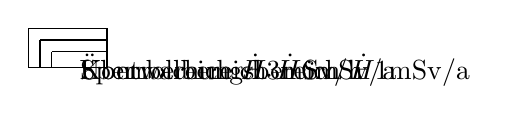
\begin{tikzpicture}
\node[right] at (1.5em , -1.5em) {Überwachungsbereich $\dot{H} \frq 1\rm mSv/a$};
\draw (0cm,0cm) -- (\masstabgrafik,0cm);  
\draw (\masstabgrafik,0cm) -- (\masstabgrafik,-0.5\masstabgrafik) ;
\draw (\masstabgrafik,-0.5\masstabgrafik) --(0cm,-0.5\masstabgrafik);
\draw (0cm,0cm) -- (0cm,-0.5\masstabgrafik) ;

\node[right] at (0.15\masstabgrafik+1.5em,-0.15\masstabgrafik -1.5em) {Kontrollbereich $\dot{H} \frq 6\rm mSv/a$};
\draw (0.15\masstabgrafik,-0.15\masstabgrafik) -- (\masstabgrafik,(-0.15\masstabgrafik);  
\draw (0.15\masstabgrafik,-0.15\masstabgrafik) -- (0.15\masstabgrafik,-0.5\masstabgrafik) ;

\node[right] at (0.3\masstabgrafik+1.5em,-0.3\masstabgrafik -1.5em) {Sperrbereich $\dot{H} \frq 3\rm mSv/h$};
\draw (0.3\masstabgrafik,-0.3\masstabgrafik) -- (\masstabgrafik,-0.3\masstabgrafik);  
\draw (0.3\masstabgrafik,-0.3\masstabgrafik) -- (0.3\masstabgrafik,-0.5\masstabgrafik) ;
\end{tikzpicture}
\end{center}
}%
\begin{description}
\parbox{\textwidth}{%
\item[Überwachungsbereich:] $\dot{H} \frq 1\rm mSv/a$ bei 2000 h/a oder Aufenthaltszeit/a.\\
Überwachungsbereiche sind nicht zum Kontrollbereich gehörende betriebliche Bereiche, in denen Personen im Kalenderjahr eine effektive Dosis von mehr als 1 Millisievert oder höhere Organdosen als 15 Millisievert für die Augenlinse oder 50 Millisievert für die Haut, die Hände, die Unterarme, die Füße und Knöchel erhalten können.
\begin{itemize}
\itemsep0pt
\item dem Betrieb dienende Aufgabe
\item Patienten, helfende Person
\item Azubi (Ausbildungsziel!)
\item Besucher
\end{itemize}
}%

\parbox{\textwidth}{%
\item[Kontrollbereich:] $\dot{H} \frq 6\rm mSv/a$bei 2000 h/a oder Aufenthaltszeit/a.\\
Kontrollbereiche sind Bereiche, in denen Personen im Kalenderjahr eine effektive Dosis von mehr als 6 Millisievert oder höhere Organdosen als 45 Millisievert für die Augenlinse oder 150 Millisievert für die Haut, die Hände, die Unterarme, die Füße und Knöchel erhalten können.
\begin{itemize}
\itemsep0pt
\item dem Betrieb dienende Aufgabe
\item Patienten, helfende Person mit Zustimmung FK
\item Azubi (Ausbildungsziel!)
\item Bei Schwangeren mit Zustimmung SSB +...
\item Dosimeter tragen!
\end{itemize}
}%

\parbox{\textwidth}{%
\item[Sperrbereich:] $\dot{H} \frq 3\rm mSv/h$\\
Sperrbereiche sind Bereiche des Kontrollbereiches, in denen die Ortsdosisleistung höher als 3 Millisievert durch Stunde sein kann.\\
\wichtig{Bei Röntgen kein Sperrbereich}
\begin{itemize}
\itemsep0pt
\item dem Betrieb dienende Aufgabe mit Zustimmung FK
\item Patienten, helfende Person mit zustimmung FK
\end{itemize}
}%
\end{description}


%%%%%%%%%%%%%
% Ortsdosis %
%%%%%%%%%%%%%
\section{Ortsdosis}
ICRU-Kugel: Kugel \O~300mm aus gewebeäquivalent.\\
\wichtig{Umgebungs}-Äquivalentdosis $H^{*}_{(10)}$ in 10mm Tiefe\\
\wichtig{Richtungs}-Äquivalentdosis $H^{'}_{(0.07)}$ in 0.07mm Tiefe

%%%%%%%%%%%%%%%%%%%%%%%%%%%%%%%%%%%%%%%%%%%%%%%%%%%%%
% Strahlenschutz- Verantwortlicher vs. Beauftragter %
%%%%%%%%%%%%%%%%%%%%%%%%%%%%%%%%%%%%%%%%%%%%%%%%%%%%%
\section{Strahlenschutz- Verantwortlicher vs. Beauftragter}
\begin{tabularx}{\textwidth}{X X}
Verantwortlicher	& Beauftragter\\
\begin{itemize}
\itemsep0pt
\item Organisation der Strahlenschutzes
\item Bestellung der Strahlen\-schutz\-beauftragten
\item Verantwortung für die Einhaltung aller Strahlenschutz\-vorschriften
\end{itemize}&
\begin{itemize}
\itemsep0pt
\item Leitung oder Beaufsichtigung bei Umgang mit radioaktiven Stoffen
\item Einhaltung aller Strahlenschutz\-vorschriften entsprechend seinem Entscheidungs\-bereich
\end{itemize}
\\
\end{tabularx}

%%%%%%%%%%%%%%%%%%%%%%%%%%
% Strahlenschutz Planung %
%%%%%%%%%%%%%%%%%%%%%%%%%%
\section{Strahlenschutz Planung}
\fwichtig{Für Strahlenqualität i: $s_{\rm i} = z_{\rm i}\cdot log_{10}\cdot\left(\bruch{W_{\rm A} U T k_{\rm i} q_{\rm i}}{H_{\rm w}}\right)$\\
\begin{tabular}{r l}
$s_{\rm i}$ & Schichtdicke\\
$z_{\rm i}$ & Zentelwerts Dicke \\
$W_{\rm a}$ & Betriebsbelastung\\
$U$ & Richtugsfaktor\\
$T$ & Aufenthaltsfaktor\\
$k_{\rm i}$ & Reduktionsfaktor = $\frac{a_0^2}{a^2}$, $a_0$: Fokusp. - Isozentrum, $a$: Fokusp. - Aufenthaltsort\\
$q_{\rm i}$ & Strahlungsqualität \\
$H_{\rm W}$ & zugelassene Wochendosis\\
\end{tabular}
}

%%%%%%%%%%%%%%%%%%%%%%%%%%%%%%%%
% Dekontamination beim Menschen%
%%%%%%%%%%%%%%%%%%%%%%%%%%%%%%%%
\section{Dekontamination beim Menschen}
\begin{enumerate}
\itemsep-1pt
\item Kontaminieret Kleidung entfernen und Verpacken
\item Messen
\item Waschen
\item Abbrechen wenn Aktivität pro Hautfläche $<$ 10 $\rm\frac{GB}{cm^2}$
\item zurück zu 2.
\end{enumerate}
\fwichtig{Kontamination des Messgeräts verhindern!}

%%%%%%%
% PSE %
%%%%%%%
%\section{PSE}
%\includegraphics[angle=90,width=0.95\textwidth]{PSE.pdf}

\end{document}

